% Copyright 2004 by Till Tantau <tantau@users.sourceforge.net>.
%
% In principle, this file can be redistributed and/or modified under
% the terms of the GNU Public License, version 2.
%
% However, this file is supposed to be a template to be modified
% for your own needs. For this reason, if you use this file as a
% template and not specifically distribute it as part of a another
% package/program, I grant the extra permission to freely copy and
% modify this file as you see fit and even to delete this copyright
% notice. 

\documentclass{beamer}
\usepackage{amsmath, amssymb, graphics, setspace, breqn, graphicx}
% There are many different themes available for Beamer. A comprehensive
% list with examples is given here:
% http://deic.uab.es/~iblanes/beamer_gallery/index_by_theme.html
% You can uncomment the themes below if you would like to use a different
% one:
%\usetheme{AnnArbor}
%\usetheme{Antibes}
%\usetheme{Bergen}
%\usetheme{Berkeley}
%\usetheme{Berlin}
%\usetheme{Boadilla}
%\usetheme{boxes}
%\usetheme{CambridgeUS}
%\usetheme{Copenhagen}
%\usetheme{Darmstadt}
%\usetheme{default}
%\usetheme{Frankfurt}
%\usetheme{Goettingen}
%\usetheme{Hannover}
%\usetheme{Ilmenau}
%\usetheme{JuanLesPins}
%\usetheme{Luebeck}
\usetheme{Madrid}
%\usetheme{Malmoe}
%\usetheme{Marburg}
%\usetheme{Montpellier}
%\usetheme{PaloAlto}
%\usetheme{Pittsburgh}
%\usetheme{Rochester}
%\usetheme{Singapore}
%\usetheme{Szeged}
%\usetheme{Warsaw}

\title{Fonction de Green et \'equation de Dyson}

% A subtitle is optional and this may be deleted

\author{ABRIBAT Cl\'ement \and DAVY L\'eo \and KAOUAH Mohamed}
% - Give the names in the same order as the appear in the paper.
% - Use the \inst{?} command only if the authors have different
%   affiliation.

\institute[Universities of Somewhere and Elsewhere] % (optional, but mostly needed)
{
  
  L1 Parcours sp\'ecial}
% - Use the \inst command only if there are several affiliations.
% - Keep it simple, no one is interested in your street address.

\date{Soutenance Projet, 2017}
% - Either use conference name or its abbreviation.
% - Not really informative to the audience, more for people (including
%   yourself) who are reading the slides online

\subject{Fonction de Green et \'equation de Dyson}
% This is only inserted into the PDF information catalog. Can be left
% out. 

% If you have a file called "university-logo-filename.xxx", where xxx
% is a graphic format that can be processed by latex or pdflatex,
% resp., then you can add a logo as follows:

% \pgfdeclareimage[height=0.5cm]{university-logo}{university-logo-filename}
% \logo{\pgfuseimage{university-logo}}

% Delete this, if you do not want the table of contents to pop up at
% the beginning of each subsection:
\AtBeginSubsection[]
{
  \begin{frame}<beamer>{Plan}
    \tableofcontents[currentsection,currentsubsection]
  \end{frame}
}

% Let's get started
\begin{document}

\begin{frame}
  \titlepage 
\end{frame}

\begin{frame}{Outline}
  \tableofcontents
  % You might wish to add the option [pausesections]
\end{frame}

% Section and subsections will appear in the presentation overview
% and table of contents.
\section{Int\'er\^et de la fonction de Green}

\subsection{Spectroscopie}
\begin{frame}
 test6
\end{frame}
  


\subsection{Photo\'emission et photo\'emission inverse}
\begin{frame}
 \begin{figure}
\caption{Sch\'ema photoemission et photoemission inverse}
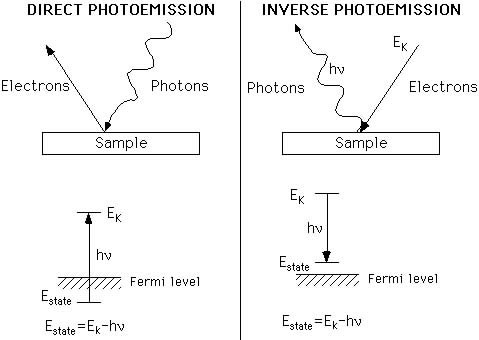
\includegraphics[width = 85mm]{photoem.jpg}
\label{solb}
\end{figure}
\end{frame}

% You can reveal the parts of a slide one at a time
% with the \pause command:

\subsection{\'Etude avec $\Psi$}



\begin{frame}
Fonction d'onde avec N corps :
\begin{equation}
 \Psi(\vec{r_1}, \vec{r_2}, ..., \vec{r_N})
\end{equation}
\begin{equation}
 \vec{r_i} = (x_i, y_i, z_i, t_i)
\end{equation}
Dans les solides \'etudi\'es il y a environ $10^{23}$ corps.
\end{frame}







\begin{frame}
 \begin{equation}
 \langle \Psi_0 | T \Psi_H (r_1, t_1) \Psi_H^\dagger (r_2, t_2) | \Psi_0 \rangle = G(\vec{r_1} t_1, \vec{r_2}  t_2)
\end{equation}
$\Psi_H^\dagger$ et $\Psi_0$ correspondent respectivement à une "destruction" et une "construction" d'un \'electron
Avec $T$ la ``time-ordering function'' d\'efinie comme suit :
\begin{equation}
 T{A(r_1)B(r_2)} := \theta(t_1 - t_2)A(r_1)B(r_2) \pm \theta(t_2 - t_1)B(r_2) A(r_1)
\end{equation}
Avec $\theta$ la fonction de Heaviside d\'efinie comme suit :

\begin{equation}
\theta(t) = 
\left\{ \begin{array}{rl}
 0 &\ \text{si }x <0\\
 1 &\ \text{si }x \geq 0
\end{array} \right.
\end{equation}


\end{frame}


\begin{frame}
 \begin{figure}
\caption{Spectre obtenu apr\`es r\'esolution de l'\'equation de Dyson}
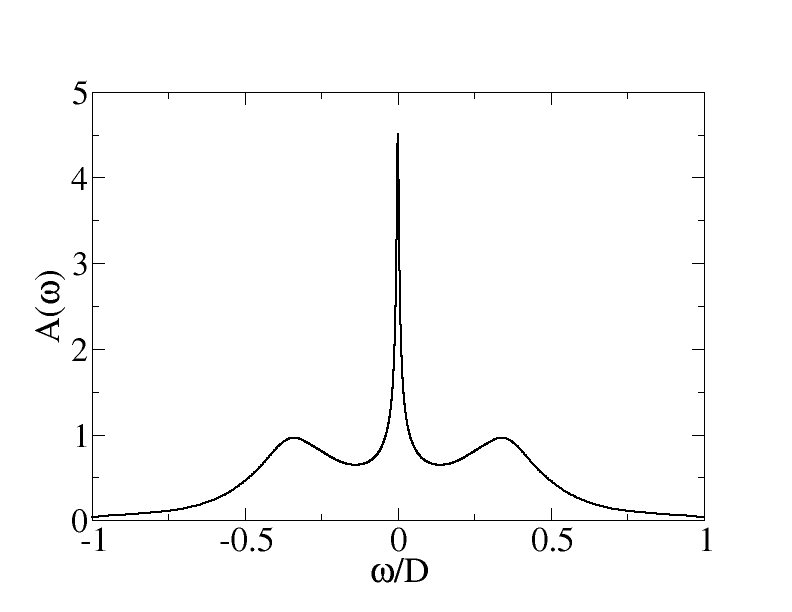
\includegraphics[width = 85mm]{spectre.png}
\label{solb}
\end{figure}
\begin{equation}
 A = \frac{1}{\pi}Im(G)
\end{equation}
\end{frame}

\section{R\'esolution}

\subsection{Pr\'esentation de l'\'equation de Dyson}

\begin{frame}
\begin{equation}
	G = G_0 + G_0 \Sigma[G] G
\end{equation}
Avec $G$ la fonction de Green qui repr\'esente le syst\`eme, $G_0$ le syst\`eme a l'\'etat initial qui est mesur\'e, et $\Sigma$ une fonctionnelle qui correspond a l'\'energie propre du syst\`eme.
$\Sigma$ s'\'ecrit :
\begin{equation}
	\Sigma[G] = \Sigma_{Hartree}[G] + \Sigma_{XC}[G]
\end{equation}

\end{frame}


\begin{frame}
 \begin{equation}
	\Sigma_{Hartree}[G] = \int \rho(r) \frac{1}{\mid r - r'\mid }\mathrm{d}r' 
\end{equation}
avec $v_c$ qui correspond au potentiel coulombien, $\rho(r)$ correspond a la densit\'e \'electronique, et $r-r'$
qui correspond à l'int\'eraction coulombienne.
\begin{equation}
	v_c =  \frac{1}{\mid r - r'\mid }
\end{equation}
\end{frame}

\begin{frame}
 \begin{equation}
	\Sigma_{XC} = G \Gamma[G] v_c
\end{equation}
\begin{equation}
	\Gamma[G] = 1 + G^2 \frac{\mathrm{d} \Sigma_{XC}[G]}{\mathrm{d}G} \Gamma[G]
\end{equation}
\end{frame}
\begin{frame}
 \begin{equation}
	\Sigma \longrightarrow S
\end{equation}
\begin{equation}
	G \longrightarrow y
\end{equation}
\begin{equation}
	\Gamma \longrightarrow g
\end{equation}
\begin{equation}
	v_c \longrightarrow u
\end{equation}

L'\'equation de Dyson devient donc
\begin{equation}
\label{dyson}
	y = y_0 + y_0 S(y) y
\end{equation}
\end{frame}
\subsection{R\'esolution dans une premi\`ere approximation}
\begin{frame}
 \'Etude avec $g^0 = 1$
\begin{equation}
 S_{Hartree}(y) = -uy
\end{equation}
 \begin{equation}
 S_{XC}(y) = \frac{1}{2} u y g^0(y) = \frac{1}{2} u y
\end{equation}
\begin{equation}
 y = y_0 + y_0 (\frac{-1}{2} u y) y
\end{equation}
\begin{equation}
 y = y_0 - y_0 \frac{1}{2} u y^2
\end{equation}
\end{frame}


\begin{frame}
 \begin{equation}
 \Delta = 1 + 2 u y_0^2
\end{equation}
On a donc $\Delta > 0 $, on obtient donc les deux solutions suivantes.
\begin{equation}
 y_1 = \frac{1 + \sqrt{1 + 2 u y_0 ^2}}{- u y_0}
\end{equation}
Et 
\begin{equation}
 y_2 = \frac{1 - \sqrt{1 + 2 u y_0^2}}{- u y_0}
\end{equation}
On peut r\'e\'ecrire les solutions pr\'ecedentes de la mani\`eresuivante:
\begin{equation}
 y_1/y_0 = Y^0_1 = \frac{-1-\sqrt{1 + 2 V}}{V}
\end{equation}
Et 
\begin{equation}
 y_2/y_0 = Y^0_2 = \frac{-1 + \sqrt{1 + 2V}}{V}
\end{equation}
\end{frame}

\begin{frame}
\begin{figure}
\caption{Comparaison entre la solution exacte (bleu) et $Y^0_2$ (orange)}
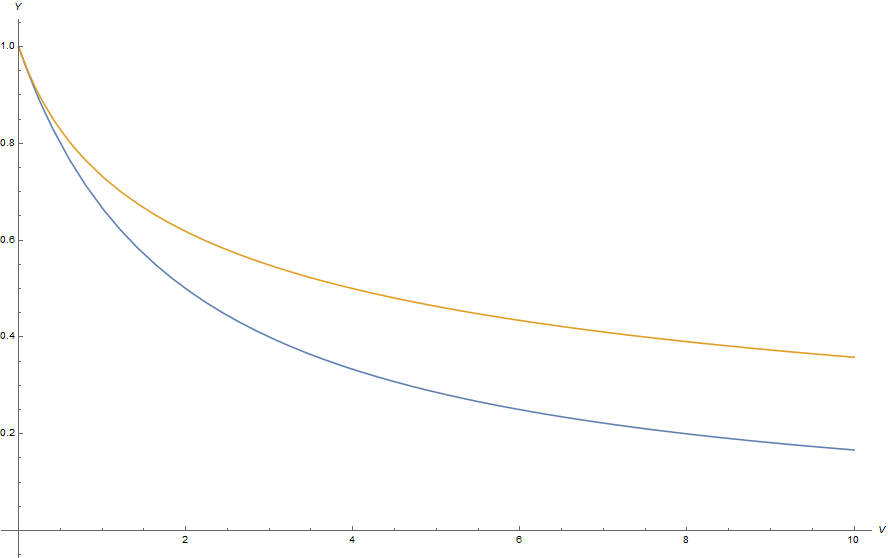
\includegraphics[width = 80mm]{CourbesPhys2.png}
\label{solb}
\end{figure}
\end{frame}
\subsection{R\'esolution dans une seconde approximation}
\begin{frame}
\begin{equation} 
\label{gamma} 
	g^1(y) = 1 + y^2 \frac{dS_{XC}(y)}{dy} 
\end{equation}

\begin{equation} 
\label{XC_dev}
	S_{XC}(y) = \frac{1}{2} u y (1 + y^2 \frac{dS_{XC}(y)}{dy})
\end{equation}
\begin{equation} 
\label{XC_prime} 
	\frac{dS_{XC}(y)}{dy} = \frac{d(\frac{1}{2} u y )}{y} = \frac{1}{2} u 
\end{equation}
On combine maintenant les \'equations \ref{XC_dev}  et \ref{XC_prime}.
\begin{equation}
\label{XC_final} 
	S_{XC}(y) = \frac{1}{2} u y + \frac{1}{4} u^2 y^3 
\end{equation} 
\end{frame}


\begin{frame}
 \begin{equation}
	\frac{1}{4} u^2 y_0 y^4 -\frac{1}{2} u y_0 y^2 - y + y_0 = 0
\end{equation}
\begin{equation}
     -\frac{1}{2} V Y^2 +\frac{1}{4} V^2 Y^4 -Y +1 = 0
\end{equation}
\begin{equation}
 a y^4 + b y^3 + c y^2 + d y + e = 0
\end{equation}
\newline
Avec $a = \frac{1}{4}V^2$,$b = 0$, $c=\frac{-1}{2}V$, $d = -1$, $e=1$ .
\end{frame}

\begin{frame}
\begin{align*}
\label{Delta}
 \Delta = 256a^3 e^3 - 192 a^2bde^2 - 128 a^2 c^2 e^2 + 144a^2cd^2e - 27a^2d^4\\ 
 + 144 ab^2ce^2 - 6ab^2d^2e - 80abc^2de + 18abcd^3 + 16ac^4e\\
 -4ac^3d^2-27b^4e^2+18b^3cde - 4b^3d^3 - 4b^2c^3e+b^2c^2d^2
 \end{align*}
\begin{equation}
 \Delta = 256a^3 e^3 - 128 a^2 c^2 e^2 + 144a^2cd^2e - 27a^2d^4 + 16ac^4e -4ac^3d^2
\end{equation}

\begin{equation}
 \Delta = 2V^6 - 5V^5 - \frac{27}{16} V^4 + \frac{1}{8}V^6
\end{equation}
\begin{equation}
\label{P}
 P = 8ac - 3b^2 = -V^3
\end{equation}
\begin{equation}
 D = 64a^3e -16a^2c^2 + 16ab^2c - 16a^2bd -3b^4
\end{equation}
\begin{equation}
\label{D}
 D = V^6
\end{equation}
\end{frame}
\begin{frame}
\begin{equation}
\left\{ \begin{array}{rl}
Y^1_{1} = - S - \frac{1}{2}\sqrt{-4S^2+\frac{4}{V}-\frac{4}{V^2 S}}\\
Y^1_{2} = - S + \frac{1}{2}\sqrt{-4S^2+\frac{4}{V}-\frac{4}{V^2 S}}\\
Y^1_{3} = + S - \frac{1}{2}\sqrt{-4S^2+\frac{4}{V}-\frac{4}{V^2 S}}\\
Y^1_{4} = + S + \frac{1}{2}\sqrt{-4S^2+\frac{4}{V}-\frac{4}{V^2 S}}
\end{array} \right.
\end{equation} 
\end{frame}

\begin{frame}
\begin{dmath}
Y^1_{1,2,3,4} = \pm\frac{1}{2} \left(\frac{4}{3 V}+\frac{26}{3 \left(27 V^2+35 V^3+3 \sqrt{3} \sqrt{27 V^4+70 V^5-36 V^6}\right)^{1/3}}\newline+\frac{2
\left(27 V^2+35 V^3+3 \sqrt{3} \sqrt{27 V^4+70 V^5-36 V^6}\right)^{1/3}}{3 V^2}\right)^{\frac{1}{2}} \newline
\pm\frac{1}{2} \left(\frac{8}{3 V}-\frac{26}{3 \left(27 V^2+35 V^3+3
\sqrt{3} \sqrt{27 V^4+70 V^5-36 V^6}\right)^{1/3}}
\newline
-\frac{2 \left(27 V^2+35 V^3+3 \sqrt{3} \sqrt{27 V^4+70 V^5-36 V^6}\right)^{1/3}}{3 V^2}-
\newline
\frac{8}{V^2
\sqrt{\frac{4}{3 V}+\frac{26}{3 \left(27 V^2+35 V^3+3 \sqrt{3} \sqrt{27 V^4+70 V^5-36 V^6}\right)^{1/3}}+\frac{2 \left(27 V^2+35 V^3+3 \sqrt{3} \sqrt{27
V^4+70 V^5-36 V^6}\right)^{1/3}}{3 V^2}}}\right)^{\frac{1}{2}}
\end{dmath}
\end{frame}

\begin{frame}
 \begin{figure}
\caption{Trac\'e des deux solutions r\'eelles, $Y^1_N = f_N(V)$}
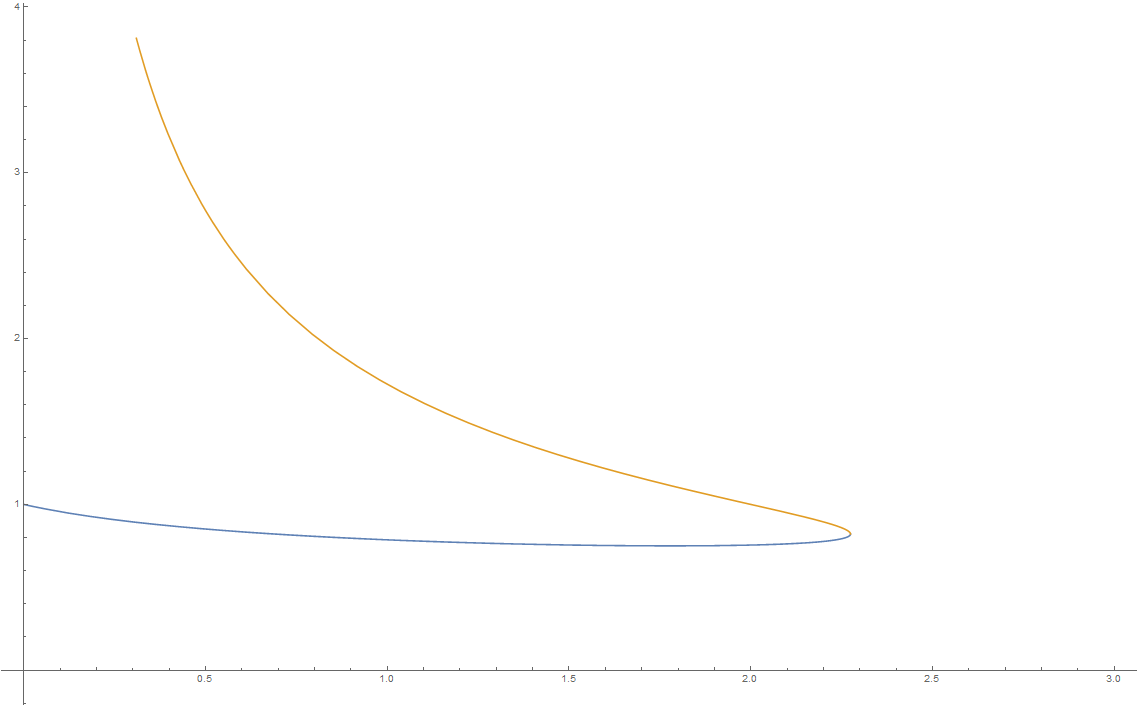
\includegraphics[width = \textwidth]{Courbes2.png}
\label{solb}
\end{figure}

\end{frame}

\begin{frame}
\begin{figure}
\caption{Comparaison entre la solution exacte (bleu), $Y^0_2$ (orange) et $Y^1_3$ (vert)}
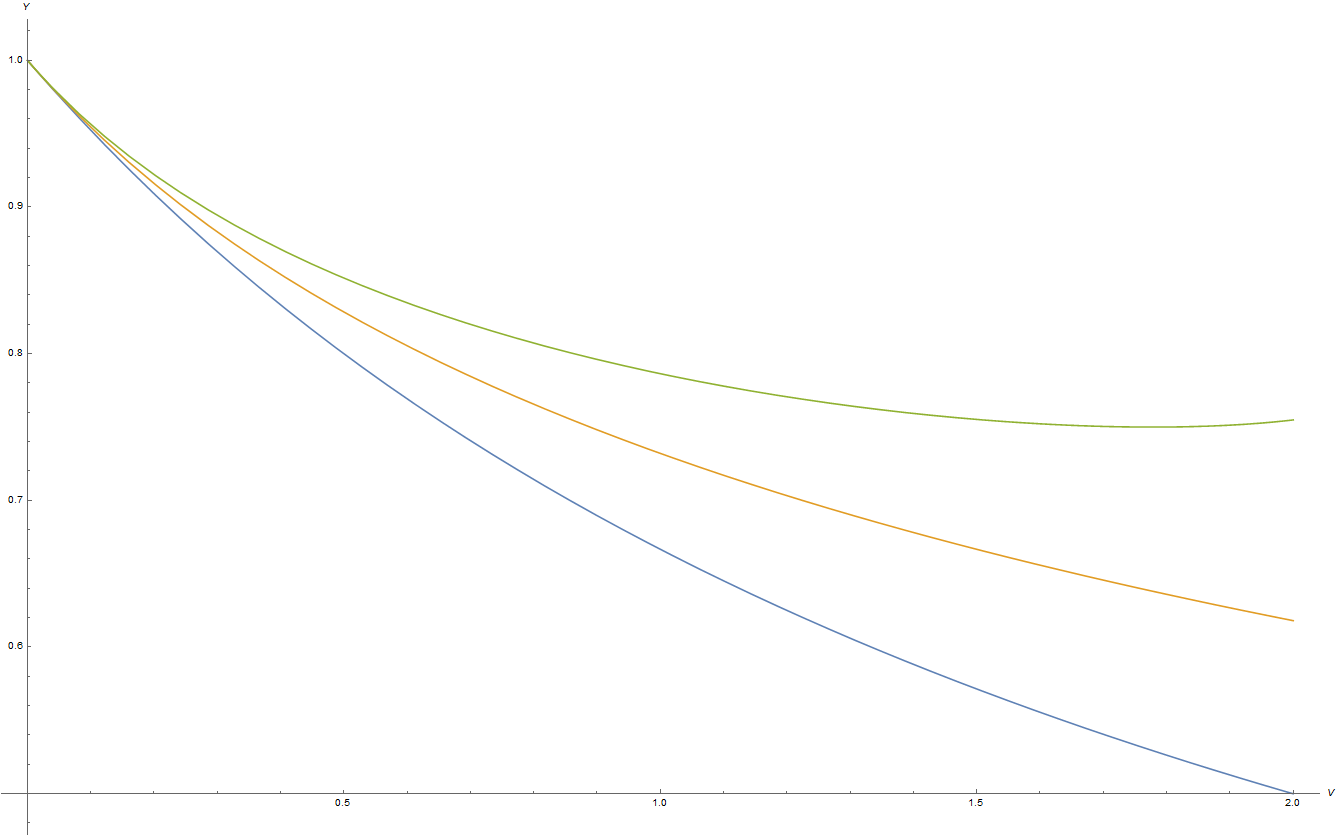
\includegraphics[width = 80mm]{CourbesPhys3.png}
\label{solb}
\end{figure}
\end{frame}
% All of the following is optional and typically not needed. 
\appendix
\section<presentation>*{\appendixname}
\subsection<presentation>*{For Further Reading}

\begin{frame}[allowframebreaks]
  \frametitle<presentation>{For Further Reading}
    
  \begin{thebibliography}{10}
    
  \beamertemplatebookbibitems
  % Start with overview books.

  \bibitem{Author1990}
    A.~Author.
    \newblock {\em Handbook of Everything}.
    \newblock Some Press, 1990.
 
    
  \beamertemplatearticlebibitems
  % Followed by interesting articles. Keep the list short. 

  \bibitem{Someone2000}
    S.~Someone.
    \newblock On this and that.
    \newblock {\em Journal of This and That}, 2(1):50--100,
    2000.
  \end{thebibliography}
\end{frame}

\end{document}


